\section{Introduction}
SeaQuest is a fixed-target experiment utilizing the 120 GeV proton beam from 
the Fermilab Main Injector. Details of the SeaQuest spectrometer can be found 
in Ref.\ \cite{aidala2019}. A schematics of the spectrometer is shown in Fig.\ 
\ref{fig:spectrometer}. The target system consists of seven interchangeable 
targets, including a flask with liquid hydrogen, a flask with liquid deuterium,
an empty flask (vacuum), solid carbon, iron, and tungsten targets as well as a 
space with no target (air). The targets are interchanged periodically to reduce 
systematic uncertainties in the measured cross section ratios for different 
targets.

The spectrometer consists of two magnets and four tracking stations. FMag, 
placed 104 cm downstream the target, is a 5 m solid iron magnet that acts as 
the beam dump as well as a focusing magnet. It is then followed by the first 
tracking stations. Stations 1, 2 and 3 each consists of plastic scintillator 
hodoscopes and drift chambers. An open air dipole magnet (KMag) is placed 
between station 1 and station 2. The vertical magnetic field from both magnets 
bends the muons horizontally, allowing the measurement of the momentum of the 
muons. Downstream of station 3, there is a 1 m iron wall acting as a hadron 
absorber. Station 4 is located behind the hadron absorber and acts as a muon 
identifier. Station 4 consists of a hodoscope array and 4 layers of 
proportional tube planes. Tracks that pass through the hadron absorber and 
produce hits on station 4 are assumed to be from muons. 

\begin{figure}[h!]
    \centering
    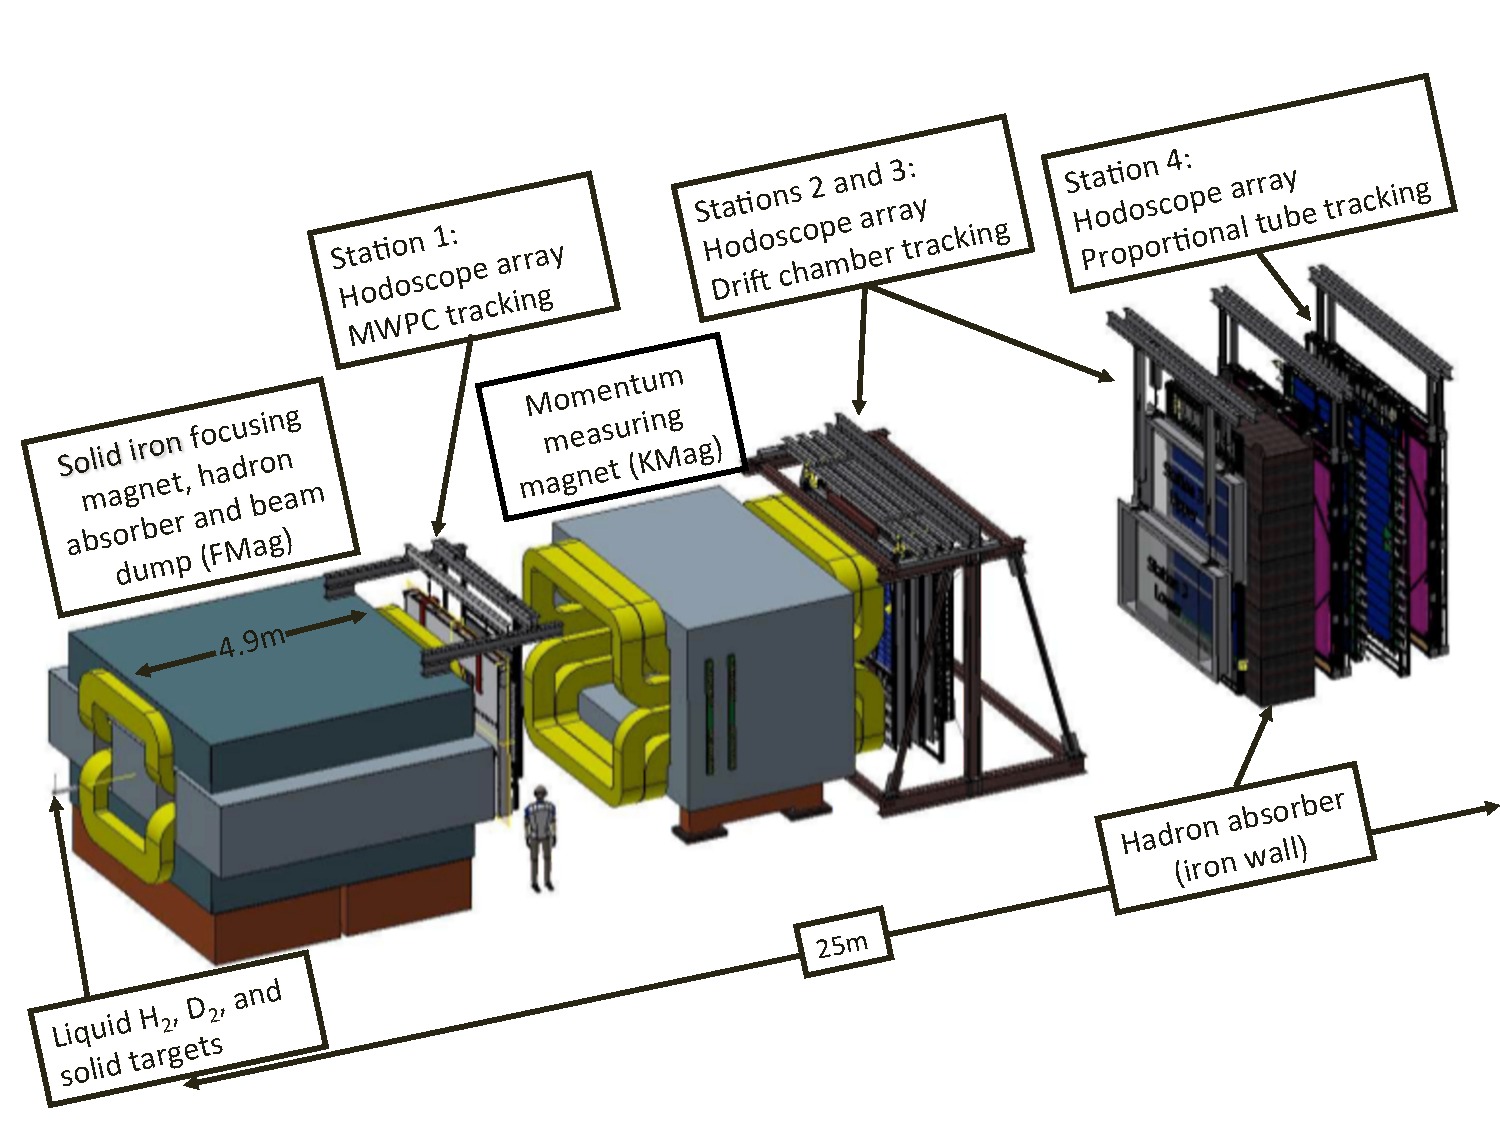
\includegraphics[width=0.6\linewidth]{SeaQuestSpectrometer}
    \caption{schematics of the SeaQuest spectrometer. Taken from Ref.\ 
		\cite{aidala2019}}
    \label{fig:spectrometer}
\end{figure}
\
